\chapter{Current and Proposed Work}

Much of the current work have been devoted to building the tools necessary to proceed to more complicated problems in the future.
The thermodynamics package discussed in \cref{Appendix:THProperties} was a large effort in-itself.
The transient solver for the computational geometry is still a work in progress.
However, a steady-state solver for a simple, closed loop is completed and will be discussed.

\section{Steady-state Solver}\label{Section:SSSolver}

\subsection{Description of the Algorithm}
As discussed in \cref{Subsection:SpatialDiscretization}, the steady-state equations for a closed loop are singular and, therefore, not directly invertible.
However, for a closed loop, the total pressure gradient is $0$.
Therefore, knowing that the density and internal energy of the starting point will be the same (meaning the same pressure), the loop can be integrated from end to end assuming a momentum.
The pressure at the start (known) is then compared with the pressure at the end.
The pressure at the end of the integration loop is a function of the initial momentum since it governs the frictional losses.
If the end pressure is higher than the known state, there was not enough frictional pressure loss; the speed is increased and the integration is performed again.
If the end pressure is lower than the known state, there was too much frictional pressure loss; the speed is deceased and the integration is performed again.

\subsection{Test Problem}
A simple natural circulation loop is shown in \cref{Figure:SimpleNatCirc}.
The test problem is for single phase water with a pressure of $101325$ Pa and temperature of $300$ K.
The power load is $10$ kW added and removed.
Because this is a single phase problem and water is nearly incompressible, the problem is approximately solvable by hand.
Results for both the steady-state solver and the hand calculations are given in \cref{Table:ComparisonOfResults}.

While the problem is simple, it is a proof-of-concept that the solver works for single phase flow.
Multiphase with HEM is currently being investigated.

\begin{figure}[b]
    \centering
    \caption[A simple natural circulation loop]{A simple natural circulation loop for testing the steady-state solver.
        The blue and red outlines indicate cooling and heating zone, respectively. ;
        the total power added and removed is $10$ kW.
        The green dot is the known state: pressure is $101325$ Pa and temperature $300$ K.
        The numbered dot coincide in the data listed in \cref{Table:ComparisonOfResults}.}
    \label{Figure:SimpleNatCirc}%
    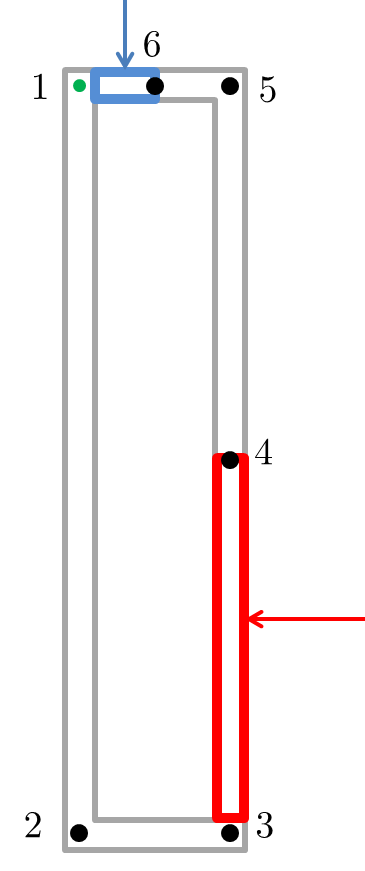
\includegraphics[height=3.5in]{SimpleNatCirc}%
\end{figure}
\begin{table}[b]%
    \centering
    \caption[Comparison between the written steady-state solver and a hand calculation]{
        Comparison between the written steady-state solver and a hand calculation for the same problem.
        The measurement points' location coincides with those in \cref{Figure:SimpleNatCirc}}
    \label{Table:ComparisonOfResults}
    \rowcolors{2}{}{Gray}
    \setstretch{1.05}
    \renewcommand{\arraystretch}{1.4}
    \begin{tabular}{ccclcclcc}
        \toprule
        \textbf{\multirow{2}{*}{Measure Point}} & \multicolumn{2}{c}{\textbf{Pressure} [kPa]}       && 
                                                  \multicolumn{2}{c}{\textbf{Temperature} [K]}      && 
                                                  \multicolumn{2}{c}{\textbf{Density} [kg/m\sups3]} \\\cmidrule(r){2-9}
                                                & Solver & Hand  && Solver & Hand  && Solver & Hand  \\\midrule
                1 & 101325 & 101325 && 300.0 & 300   && 996.6 & 996.6\\
                2 & 150192 & 150178 && 300.0 & 300   && 996.6 & 996.6\\
                3 & 150190 & 150175 && 300.0 & 300   && 996.6 & 996.6\\
                4 & 130640 & 130631 && 302.9 & 302.9 && 995.7 & 995.7\\
                5 & 101327 & 101328 && 302.9 & 302.9 && 995.7 & 995.7\\
                6 & 101326 & 101326 && 302.9 & 302.9 && 995.7 & 995.7\\\bottomrule
    \end{tabular}
\end{table}



\clearpage
\section{Proposed Work}
As was discussed in \cref{Section:Purpose}, this is the work completed for review currently.
A proposed path forward is completion of the fully transient HEM to be able to calculate the state of the system over time.
Following that, investigation into the physical phenomenon observed in the two-fluid simulations from MELCOR (\cref{Figure:RCCSFullScaleMassFlowRate,Figure:ExperimentMassFlowRateVsTime}) and experimental data.

The ultimate goal is to be able to assess, predict, and physically explain the observed stability issues of this \Acronym{RCCS} system.
When the goal is met, this work will be considered all but complete.
Time permitting (or if simply need from a theoretical perspective), investigation and possible implementation of different flow regime models and multiphase flow models may be done.

This is the work proposed for the natural circulation of the RCCS for completion of this thesis.



